\subsection*{Lato Client}

%% Slide 11.
\begin{frame}
\frametitle{Le classi ed i moduli client}
\begin{itemize}[<+->]
\item
\alert{\texttt{Avatar}}:
rappresenta l'utente nell'ambiente virtuale, mantiene
i dati relativi alla posizione attuale ed ai vicini;
\item
\alert{\texttt{Source}}:
dalla libreria
\texttt{queueinglib} simula le azioni
dell'utente nell'utilizzo del client;
\item
\alert{\texttt{DVEClient}}:
è il client vero e proprio ed è definito dal modulo \texttt{DVEClient.ned} e
dalla relativa classe \texttt{C++} che ne definisce il comportamento.
\end{itemize}
\end{frame}

%% Slide 12.
\begin{frame}[fragile]
\frametitle{Generazione di eventi}
\begin{columns}
%% Left Column
\begin{column}{0.65\textwidth}
\begin{block}{}
\begin{itemize}
\item
Ogni client è rappresentato da due moduli \alert{\texttt{Source}} e
\alert{\texttt{DVEClient}} connessi;
\item
\texttt{Source} genera dei messaggi ad intervalli regolari che vengono
interpretati come azioni;
\item
la prima azione è il login, ed avviene ad un tempo
casuale nei primi 10 secondi di simulazione.
\end{itemize}
\end{block}
\end{column}
%% Right Column
\begin{column}{0.35\textwidth}
\begin{center}
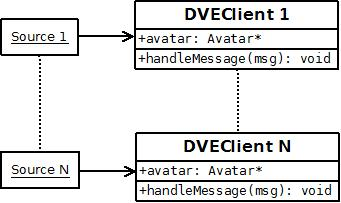
\includegraphics[scale=.45]{source.jpeg}
\end{center}
\end{column}
\end{columns}
\begin{center}
\begin{lstlisting}[title = {\texttt{omnetpp.ini}}]
DVESystem.source[*].interArrivalTime = 2s
DVESystem.source[*].startTime = uniform(0s,10s)
\end{lstlisting}
\end{center}
\end{frame}

%% Slide 13.
\begin{frame}
\frametitle{Registrazione dati e statistiche}
\begin{itemize}[<+->]
\item \textbf{Risposta del sistema}: calcola il tempo simulato di risposta
del sistema, ovvero ad ogni movimento del client misura il tempo impiegato
per notificare tutti i client coinvolti.
\item \textbf{Movimenti persi}: tiene conto dei movimenti persi di ogni client.
Quando un nuovo \texttt{job} arriva al client per effettuare un movimento, se
non è ancora arrivata la notifica (ACK) di quello precedente non è possibile
effettuare il nuovo.
\item \textbf{Movimenti nulli}: conta i movimenti non effettuati ``volutamente''
dall'utente.
\item \textbf{Movimenti}: conta i movimenti effettuati con successo.
\item \textbf{Presence Factor}: conta la ``numerosità'' della AoI, ovvero
il numero di altri avatar nella medesima zona.
\end{itemize}
\end{frame}

%% Slide 14.
\begin{frame}[fragile]
\frametitle{Registrazione dati e statistiche}
\begin{lstlisting}[title = {Modulo ned}]
simple DVEClient
{
  parameters:
    @signal[sysResponse](type="simtime_t");
    @statistic[dveResponse](...);
    @signal[presenceFactor](type="unsigned int");
    @statistic[clientPresenceFactor](...);
    ...
}
\end{lstlisting}
\begin{lstlisting}[title = {Classe \texttt{DVEClient}}]
  // Statistics.
  simtime_t timeRequest;
  simsignal_t systemResponseSignal;
  int ackReceived;
  simsignal_t presenceFactorSignal;
  unsigned int presenceFactor;
  ...
\end{lstlisting}
\end{frame}

%% Slide 15.
\begin{frame}[fragile]
\frametitle{Registrazione dati e statistiche}
\begin{lstlisting}[title = {Inizializzazione}]
  ...
  systemResponseSignal = registerSignal("sysResponse");
  presenceFactor = avatar->GetAoISize();
  WATCH(presenceFactor);
  presenceFactorSignal = registerSignal("presenceFactor");
\end{lstlisting}
\begin{lstlisting}[title = {Movimento}]
  ...
  avatar->move(x, y);
  send(move, "wanIO,o");
  timeRequest = simTime();
\end{lstlisting}
\begin{lstlisting}[title = {System Response}]
  ...
  simtime_t response = simTime() - timeRequest;
  emit(systemResponseSignal, response);
  // Movement complete: update presence factor.
  presenceFactor = avatar->GetAoISize();
  emit(presenceFactorSignal, presenceFactor);
\end{lstlisting}
\end{frame}


\subsection*{Lato Server}

%% Slide 16.
\begin{frame}
\frametitle{Le classi ed i moduli server}
\begin{itemize}[<+->]
\item
\alert{\texttt{VirtualAvatar}}:
rappresenta l'avatar all'interno
dell'ambiente virtuale gestito dal Main Server;
\item
\alert{\texttt{VirtualEnvironment}}:
``simula'' un'area in cui gli avatar possono muoversi liberamente e
senza collisioni;
\item
\alert{\texttt{MainServer}}:
è il server principale, composto dal modulo \texttt{MainServer.ned} e dalla
relativa classe \texttt{C++}, si occupa di gestire l'ambiente virtuale e la
partizione;
\item
\alert{\texttt{DVEServer}}:
sono i server di partizione, composti dal modulo \texttt{DVEServer.ned} e dalla
relativa classe \texttt{C++},
si occupano di gestire le comunicazioni con i client.
\end{itemize}
\end{frame}

%% Slide 17.
\begin{frame}[fragile]
\frametitle{Gestione del mondo}
\begin{block}{Quando un client notifica un movimento, il MainServer:}
\begin{itemize}
\item
Calcola la nuova AoI del client e notifica i nuovi vicini;
\item
Aggiorna lo stato interno del mondo (VE).
\end{itemize}
\end{block}

\begin{lstlisting}
  int* newAoi = NULL;
  unsigned int newAoiSize;
  ve_->GetAvatarAndSizeAt(x, y, &newAoi, newAoiSize);
  UpdateAoIMsg* update = new UpdateAoIMsg();
  update->setClientMoved(clientID);
  update->setX(x);
  update->setY(y);
  update->setAoiArraySize(newAoiSize);
  for (unsigned int index = 0; index < newAoiSize; index++)
  {
    update->setAoi(index, newAoi[index]);
  }
  update->setIsNeighborNotification(false);
  send(update, "lanOut");
  // Updates VA and VE.
  VirtualAvatar* avatar = connectedAvatars_[clientID];
  avatar->move(x, y);
\end{lstlisting}
\end{frame}

%% Slide 18.
\begin{frame}[fragile]
\frametitle{Sistema di notifica}
\begin{block}{Quando un client notifica un movimento, il MainServer:}
\begin{itemize}
\item
Se non ci sono vicini coinvolti manda direttamente l'ack al client;
\item
Altrimenti crea un registro per raccogliere le notifice dei vicini, l'ack
sarà inoltrato in seguito.
\end{itemize}
\end{block}

\begin{lstlisting}
  int aksRequired = (msgAoISize <= oldAoiSize) ? msgAoISize + newAoiSize
            : newAoiSize + oldAoiSize;
  if (aksRequired == 0)
  {
    // No client to be notified, send the ack to client moved.
    ACKMsg* ack_msg = new ACKMsg();
    ack_msg->setMovedID(clientID);
    send(ack_msg, "lanOut");
  }
  else
  {
    // Insert the new ack into the registry.
    Acknowledgment* ack = new Acknowledgment();
    ack->current = 0;
    ack->total = aksRequired;
    ack_registry_.insert(std::pair<int, Acknowledgment*>(clientID, ack));
  }
\end{lstlisting}
\end{frame}


\subsection*{Connessioni e rete}

%% Slide 19.
\begin{frame}[fragile]
\frametitle{Le classi ed i moduli della rete}
\begin{itemize}[<+->]
\item
\alert{\texttt{WAN}}:
rappresenta la rete internet, è composta da un modulo \texttt{WAN.ned} e
la relativa classe \texttt{C++}, si occupa di inoltrare e indirizzare i
messaggi tra client e server;
\item
\alert{\texttt{LAN}}:
è un canale definito con una latenza molto bassa per simulare le connessioni
della LAN, un anello unidirezionale.
\end{itemize}
\pause
\begin{lstlisting}[title = {DVESystem.ned}]
channel LAN extends ned.DelayChannel
{
  delay = 1ms;
}
\end{lstlisting}
\end{frame}

%% Slide 20.
\begin{frame}[fragile]
\frametitle{Simulazione del delay}
\begin{lstlisting}[title = {\texttt{omnetpp.ini}: definizione della media},
                  ]
DVESystem.wan.delayMean = 0.10s
\end{lstlisting}

\begin{lstlisting}[title = {\texttt{WAN.cc}: inizializzazione della media},
                  ]
WAN::initialize()
{
    mean = par("delayMean");
}
\end{lstlisting}

\begin{lstlisting}[title = {\texttt{WAN.cc}: tipico meccanismo di routing},
                  ]
  const char* gateName = gate->getName();
  if (strcmp(gateName, "toClient\$i") == 0)
  {
    sendDelayed(l_msg, exponential(mean), "toMainServer\$o");
  }
  else if (strcmp(gateName,"toMainServer\$i") == 0)
  {
    sendDelayed(l_msg, exponential(mean), "toClient\$o", l_msg->getID());
  }
\end{lstlisting}
\end{frame}

%% Slide 21.
\begin{frame}
\frametitle{DVE System}
\begin{columns}
%% Left Column
\begin{column}{0.5\textwidth}
\begin{block}{Un esempio di DVE System}
\begin{itemize}
\item
$1$ server principale;
\item
$3$ server di partizione;
\item
$n$ client ed i rispettivi moduli \texttt{Source};
\item
una rete lan connessa ad ogni entità;
\item
i server conessi da un canale unidirezionale.
\end{itemize}
\end{block}
\end{column}
%% Right Column
\begin{column}{0.5\textwidth}
\begin{center}
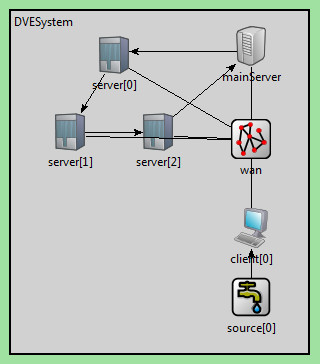
\includegraphics[scale=.45]{dvesystem.jpeg}
\end{center}
\end{column}
\end{columns}
\end{frame}
